% Εισαγωγή

\addcontentsline{toc}{chapter}{Εισαγωγή}
\chapter*{Εισαγωγή}


Το ερευνητικό αντικείμενο της παρούσας εργασίας είναι οι προβολές \textlatin{Cavalier} και \textlatin{Cabinet} σε μοναδιαίο κύβο. Συγεκριμένα, στόχος της εργασίας είναι η εμβάθυνση στις προβολές αντικειμένων σε 3Δ σκηνές και ειδικότερα η κατανόηση των πλαγίων παραλλήλων προβολών \textlatin{Cavalier} και \textlatin{Cabinet}, καθώς και η δημιουργία και εφαρμογή ενός εύχρηστου προγράμματος. \par

Αρχικά, θα αναπτυχθεί το θεωρητικό σύνολο που αφορά τις προβολές, αναλύοντας τις βασικές υποκατηγορίες αυτών και κυρίως τις πλάγιες προβολές \textlatin{Cavalier} και \textlatin{Cabinet}. Στη συνέχεια, θα προταθεί τρόπος μέτρησης μηκών προβολών των ακμών ενός μοναδιαίου κύβου, οι οποίες αρχικά είναι κάθετες προς το επίπεδο $x-y$, χρησιμοποιώντας γωνία αζιμουθίου της επιλογής μας. Κατόπιν, θα ληφθούν τα μητρώα για κάθε μία από τις πλάγιες προβολές και θα πολλαπλασιαστούν με τον πίνακα κορυφών του κύβου, θα παρατηρηθούν οι προβολές κάθετες στο επίπεδο $x-y$ και θα υπολογιστούν οι νόρμες μεταξύ των σημείων που ενώνονται σε κάθε προβολή. Ως πρότυπο της υλοποίησης αυτής δυνάμεθα να συμβουλευτούμε το πρότυπο λύσης άσκησης σχετικής με τον προσδιορισμό του μητρώου των πλαγίων προβολών που καθορίζονται με γωνίες αζιμουθίου και ανύψωσης $φ$ και $θ$, και ορίζουν τη σχέση της κατεύθυνσης προβολής προς το επίπεδο προβολής. \par

\vspace{0.5em}

\begin{figure}[h]
\centering
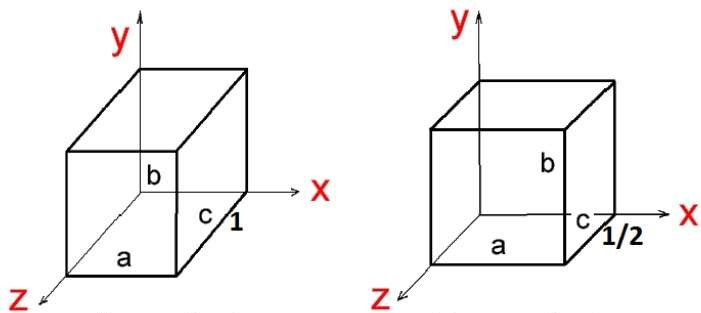
\includegraphics[width=0.6\textwidth]{images/Cavalier-Cabinet.jpg}
\caption{Προβολή \textlatin{Cavalier} (αριστερά) και προβολή \textlatin{Cabinet} (δεξιά)}
\end{figure}

Τη θεωρητική εξέταση του αντικειμένου της εργασίας θα ακολουθήσει η υλοποίηση ενός απλού προγράμματος στην προγραμματιστική γλώσσα \textlatin{C++} με τη χρήση του λογισμικού \textlatin{OpenGL}, το οποίο θα επιτρέπει στον χρήστη τη διαδραστική περιστροφή του μοναδιαίου κύβου πέριξ των αξόνων $x$, $y$ ή $z$. Αναγκαία είναι η δημιουργία τριών παραθύρων για την απεικόνιση μιας προοπτικής προβολής, της πλάγιας προβολής \textlatin{Cavalier} και της πλάγιας προβολής \textlatin{Cabinet} αντιστοίχως. \par
